\chapter{The X Window System}\label{x-chapter}

\begin{fortune}
The nice thing about standards is that there are so many of them to
choose from.\\
\raggedleft Andrew S.~Tanenbaum
\end{fortune}

\bindex{X Window System}

\xwarn This chapter only applies to those using the X Window
System.  If you encounter a screen with multiply windows, colors, or a
cursor that is only movable with your mouse, you are using X. (If
your screen consists of white characters on a black background, you
are not currently using X.  If you want to start it up, take a look at
Section~\ref{x-start-stop-section}.)

\section{Starting and Stopping the X Window System}\label{x-start-stop-section}

\subsection{Starting X}

Even if X doesn't start automatically when you login, it is possible
to start it from the regular text-mode shell prompt.  There are two
possible commands that will start X, either {\tt
  startx}\impttindex{startx} or {\tt xinit}\impttindex{xinit}. Try
{\tt startx} first. If the shell complains that no such command is
found, try using {\tt xinit} and see if X starts. If neither command
works, you may not have X installed on your system---consult local
documentation for your distribution.

If the command runs but you are eventually returned to the black
screen with the shell prompt, X is installed but not configured.
Consult the documentation that came with your distribution on how to
setup X.

\subsection{Exiting X}

% what about the possibility of the xterm being a ``login window''

Depending on how X is configured, there are two possible ways you
might have to exit X.  The first is if your window manager controls
whether or not X is running.  If it does, you'll have to exit X using
a menu (see Section~\ref{x-menus} on page~\pageref{x-menus}).  To
display a menu, click a button on the background.

The important menu entry should be ``Exit Window Manager'' or ``Exit
X'' or some entry containing the word ``Exit''.  Try to find that
entry (there could be more than one menu---try different
mouse buttons!) and choose it.  

The other method would be for a special {\tt xterm} to control X.  If
this is the case, there is probably a window labeled ``login'' or
``system xterm''.  To exit from X, move the mouse cursor into that
window and type ``exit''.

If X was automatically started when you logged in, one of these
methods should log you out.  Simply login again to return.  If you
started X manually, these methods should return you to the text mode
prompt.  (If you wish to logout, type {\tt logout} at this prompt.)

\section{What is The X Window System?}

The X Window System is a distributed, graphical method of working
developed primarily at the Massachusetts Institute of
Technology\index{Massachusetts Institute of Technology}. It has since
been passed to a consortium of vendors (aptly named ``The X
Consortium'') and is being maintained by them.

The X Window System (hereafter abbreviated as ``X''\footnote{There are
  several acceptable ways to refer to The X Window System.  A common
  though incorrect way of referring to X is ``X Windows''.}) has new
versions every few years, called releases. As of this writing, the
latest revision is X11R6, or release six. The eleven in X11 is
officially the version number but there hasn't been a new version in
many years, and one is not currently planned.

There are two terms when dealing with X that you should be familiar.
The \concept{client} is a X program. For instance, {\tt xterm} is the
client that displays your shell when you log on.  The \concept{server}
is a program that provides services to the client program. For
instance, the server draws the window for {\tt xterm} and communicates
with the user.

Since the client and the server are two separate programs, it is
possible to run the client and the server {\em on two physically
  separate machines\/}.  In addition to supplying a standard method of
doing graphics, you can run a program on a remote machine (across the
country, if you like!) and have it display on the workstation right in
front of you.

A third term you should be familiar with is the
\concept{window manager}. The window manager is a special client that
tells the server where to position various windows and provides a way
for the user to move these windows around. The server, by itself, does
nothing for the user. It is merely there to provide a buffer between
the user and the client.

\section{What's This on my Screen?}

When you first start X, several programs are started. First, the
server is started. Then, several clients are usually
started. Unfortunately, this is not standardized across various
distributions. It is likely that among these clients are a window
manager, either {\tt fvwm} or {\tt twm}, a prompt, {\tt xterm}, and a
clock, {\tt xclock}.

\begin{figure}[tbf]\label{full-x-screen}
\centering
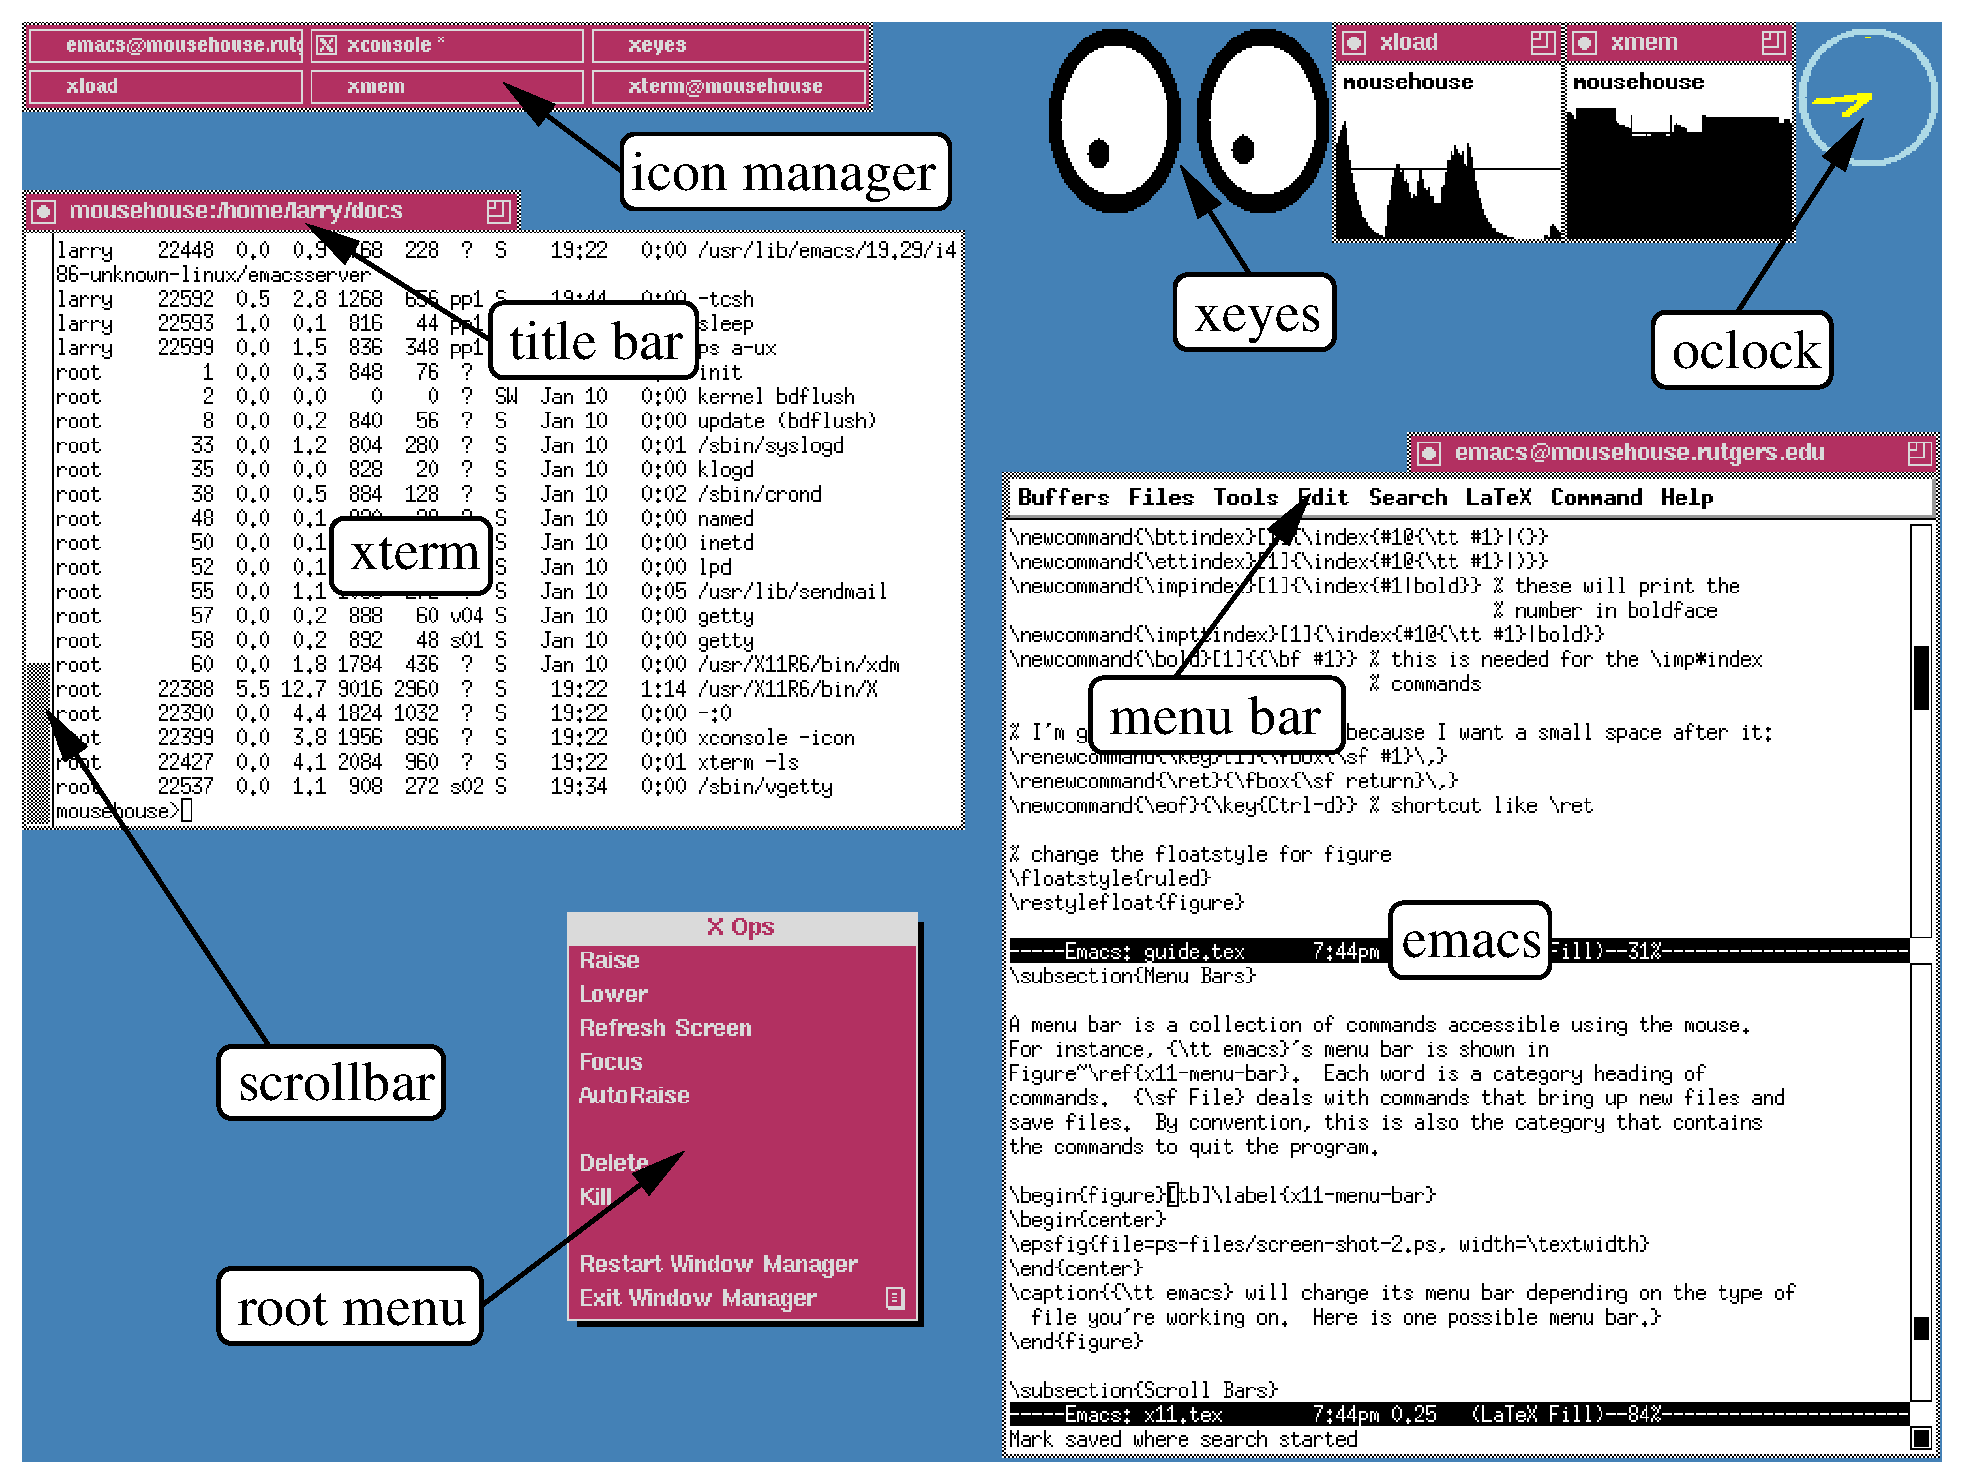
\epsfig{file=ps-files/screen-shot-5.ps, width=\linewidth}
\caption{An annotated example of a standard X screen.  In this
 example, the user is running {\tt twm}.  The standard clock has been
  replaced by a transparent clock called {\tt oclock}.}
\end{figure}

\subsection{XClock}

\begin{command}
{\tt xclock} [-digital] [-analog] [-update {\sl seconds}] [-hands {\sl
  color}]
\end{command}

I'll explain the simpliest one first: {\tt xclock}\ttindex{xclock}
functions exactly as you'd expect it would.  It ticks off the seconds,
minutes and hours in a small window.

No amounts of clicking or typing in {\tt xclock}'s window will affect
it---that's {\em all\/} it does. Or is it? In fact, there are various
different options you can give to the program to have it act in
different ways. For instance, {\tt xclock -digital} will create a
digital clock. {\tt xclock -update 1} will create a second hand that
moves every second, while {\tt -update 5} will create a second hand
that moves every 5 seconds.

For more information on {\tt xclock}'s options, consult its
manpage---{\tt man xclock}. If you're going to try running a few of
your own {\tt xclock}s, you should probably read
Section~\ref{section-multitasking} (Multitasking) to learn how to run
them in addition to your current programs.  (If you run an {\tt
  xclock} in the foreground---the usual way of running a program---and
want to get out of it, type \key{ctrl-c}.)

\subsection{XTerm} % better section name?

The window with a prompt in it (something that probably looks like
{\tt /home/larry\#}) is being controlled by a program called {\tt
  xterm}\impttindex{xterm}.  {\tt xterm} is a deceptively complicated
program.  At first glance, it doesn't seem to do much, but it actually
has to do a lot of work.  {\tt xterm} emulates a terminal so that
regular text-mode \unix\ applications work correctly.  It also
maintains a buffer of information so that you can refer back to old
commands.  (To see how to use this, look at
Section~\ref{x-scroll-bar}.)

For much of this book, we're going to be learning about the \unix\ 
command-line, and you'll find that inside your {\tt xterm} window.
In order to type into {\tt xterm}, you {\em usually\/} have to move
your mouse cursor (possibly shaped like an ``X'' or an arrow) into the
{\tt xterm} window.  However, this behavior is dependent on the window
manager.

One way of starting more programs under X is through an {\tt xterm}.
Since X programs are standard \unix\ programs, they can be run from
normal command prompts such as {\tt xterm}s.  Since running a long
term program from a {\tt xterm} would tie up the {\tt xterm} as long
as the program was running, people normally start X programs in the
background.  For more information about this, see
Section~\ref{section-multitasking}.

\section{Window Managers}

On \linux, there are two different window managers that are commonly
used.  One of them, called {\tt twm}\ttindex{twm} is short for ``Tab
Window Manager''. % this is from the manpage. is it correct?
It is larger than the other window manager usually used, {\tt fvwm}.
({\tt fvwm} stands for ``F(?) Virtual Window Manager''---the author
neglected to tie down exactly what the f stood for.)  Both {\tt twm}
and {\tt fvwm} are highly configurable, which means I can't tell you
exactly what keys do what in your particular setup.

To learn about {\tt twm}'s configuration, look at
Section~\ref{twm-config-section}. {\tt fvwm}'s configuration is
covered in Section~\ref{fvwm-config-section}.

\subsection{When New Windows are Created}

There are three possible things a window manager will do when a new
window is created.  It is possible to configure a window manager so
that an outline of the new window is shown, and you are allowed to
position it on your screen. That is called \concept{manual placement}.
If you are presented with the outline of a window, simply use the
mouse to place it where you wish it to appear and click the left mouse
button.

It is also possible that the window manager will place the new window
somewhere on the screen by itself.  This is known as 
\concept{random placement}.

Finally, sometimes an application will ask for a specific spot on the
screen, or the window manager will be configured to display certain
applications on the same place of the screen all the time. (For
instance, I specify that I want {\tt xclock} to always appear in
the upper right hand corner of the screen.)

\subsection{Focus}

The window manager controls some important things. The first thing
you'll be interested in is \concept{focus}.  The focus of the server is
which window will get what you type into the keyboard. Usually in X
the focus is determined by the position of the mouse cursor.  If the
mouse cursor is in one {\tt xterm}'s window\footnote{You can have more
  then one copy of {\tt xterm} running at the same time!}, that {\tt
  xterm} will get your keypresses.  This is different from many other
windowing systems, such as Microsoft Windows, OS/2, or the Macintosh,
where you must click the mouse in a window before that window gets
focus.  Usually under X, if your mouse cursor wanders from a
window, focus will be lost and you'll no longer be able to type there.

Note, however, that it is possible to configure both {\tt
  twm}\ttindex{twm} and {\tt fvwm}\ttindex{fvwm} so that you must
click on or in a window to gain focus, and click somewhere else to
lose it, identical to the behavior of Microsoft Windows.  Either
discover how your window manager is configured by trial and error, or
consult local documentation.

\subsection{Moving Windows}

Another very configurable thing in X is how to move windows around.
In my personal configuration of {\tt twm}, there are three different
ways of moving windows around.  The most obvious method is to move the
mouse cursor onto the \concept{title bar} and drag the window around
the screen. Unfortunately, this may be done with any of the left,
right, or middle buttons\footnote{Many PCs have only two button mice.
  If this is the case for you, you should be able to emulate a middle
  button by using the left and right buttons simultaneously.}. (To
drag, move the cursor above the title bar, and hold down on the button
while moving the mouse.)  Most likely, your configuration is
set to move windows using the \emph{left} mouse buttons.

Another way of moving windows may be holding down a key while dragging
the mouse. For instance, in {\em my\/} configuration, if I hold down
the \key{Alt} key, move the cursor above a window, I can drag the
window around using the left mouse button.

Again, you may be able to understand how the window manager is
configured by trial and error, or by seeing local
documentation. Alternatively, if you want to try to interpret the
window manager's configuration file, see
Section~\ref{twm-config-section} for {\tt twm}\ttindex{twm} or
Section~\ref{fvwm-config-section} for {\tt fvwm}\ttindex{fvwm}.

\subsection{Depth}

Since windows are allowed to overlap in X, there is a concept of
\concept{depth}.  Even though the windows and the screen are both two
dimensional, one window can be in front of another, partially or
completely obscuring the rear window.

There are several operations that deal with depth:
\begin{itemize}
\item {\bf Raising} the window, or bringing a window to the front.
  This is usually accomplished by clicking on a window's title bar
  with one of the buttons.  Depending on how the window manager is
  configured, it could be any one of the buttons. (It is also possible
  that more then one button will do the job.)

\item {\bf Lowering} the window, or pushing the window to the back.
  This can generally be accomplished by a different click in the title
  bar. It is also possible to configure some window managers so that
  one click will bring the window foward if there is anything over it,
  while that same click will lower it when it is in the front.

\item {\bf Cycling} through windows is another operation many window
  managers allow. This brings each window to the front in an orderly
  cycle.  
\end{itemize}

\subsection{Iconization}

There are several other operations that can obscure windows or hide
them completely. First is the idea of ``iconization''. Depending on
the window manager, this can be done in many different ways. In {\tt
  twm}, many people configure an {\bf icon manager}\index{icon
  manager}. This is a special window that contains a list of all the
other windows on the screen.  If you click on a name (depending on the
setup, it could be with any of the buttons!) the window
disappears---it is iconified.  The window is still active, but you
can't see it.  Another click in the icon manager restores the window
to the screen.

This is quite useful.  For instance, you could have remote {\tt
  xterm}s to many different computers that you occasionally use.
However, since you rarely use all of them at a given time, you can
keep most of the {\tt xterm} windows iconified while you work with a
small subset. The only problem with this is it becomes easy to
``lose'' windows. This causes you to create new windows that duplicate
the functionality of iconified windows.

Other window managers might create actual icons across the bottom of
the screen, or might just leave icons on the root
window.\glossary{root window}

\subsection{Resizing}

There are several different methods to resize windows under X.  Again,
it is dependent on your window manager and exactly how your window
manager is configured.  The method many Microsoft Windows users are
familiar with is to click on and drag the border of a window.  If your
window manager creates large borders that change how the mouse cursor
looks when it is moved over them, that is probably the method used to
resize windows.

Another method used is to create a ``resizing'' button on the
titlebar.  In Figure~\ref{full-x-screen}, a small button is visible on
the right of each titlebar.  To resize windows, the mouse is moved
onto the resize button and the left mouse button is held down.  You
can then move the mouse outside the borders of the window to resize
it.  The button is released when the desired size has been reached.

\subsection{Maximization}

Most window managers support maximization.  In {\tt twm}, for
instance, you can maximize the height, the width, or both dimensions
of a window. This is called ``zooming'' in {\tt twm}'s language
although I prefer the term maximization.  Different applications
respond differently to changes in their window size. (For instance,
{\tt xterm} won't make the font bigger but will give you a larger
workspace.)

Unfortunately, it is extremely non-standard on how to maximize windows.

\subsection{Menus}\label{x-menus}

Another purpose for window managers is for them to provide menus for
the user to quickly accomplish tasks that are done over and over.  For
instance, I might make a menu choice that automatically launches Emacs
or an additional {\tt xterm} for me. That way I don't need to type in
an {\tt xterm}---an especially good thing if there aren't any running
{\tt xterm}s that I need to type in to start a new program!

In general, different menus can be accessed by clicking on the root
window, which is an immovable window behind all the other ones. By
default, it is colored gray, but could look like
anything.\footnote{One fun program to try is called {\tt
    xfishtank}\ttindex{xfishtank}.  It places a small aquarium in the
  background for you.} To try to see a menu, click and hold down a
button on the desktop. A menu should pop up. To make a selection, move
(without releasing the mouse button) the cursor over one of the items
any then release the mouse button.

\section{X Attributes}

There are many programs that take advantage of X. Some programs, like
{\tt emacs}\ttindex{emacs}, can be run either as a text-mode program
{\em or\/} as a program that creates its own X window. However, most X
programs can only be run under X.

\subsection{Geometry}\index{X Window System!geometry}

There are a few things common to all programs running under X.  In X, the
concept of {\bf geometry} is where and how large a window is.  A
window's geometry has four components:
\begin{itemize}
\item The horizontal size, usually measured in pixels. (A pixel is the
  smallest unit that can be colored. Many X setups on Intel PCs have
  1024 pixels horizontally and 768 pixels vertically.) Some
  applications, like {\tt xterm} and {\tt emacs}, measure their size in
  terms of number of characters they can fit in the window. (For
  instance, eighty characters across.)
\item The vertical size, also usually measured in pixels. It's
  possible for it to be measured in characters.
\item The horizontal distance from one of the sides of the screen. For
  instance, {\tt +35} would mean make the left edge of the window
  thirty-five pixels from the left edge of the screen. On the other
  hand, {\tt -50} would mean make the right edge of the window fifty
  pixels from the right edge of the screen.  It's generally impossible to start
  the window off the screen, although a window can be moved off the
  screen.  (The main exception is when the window is very large.)
\item The vertical distance from either the top or the bottom. A
  positive vertical distance is measured from the top of the screen; a
  negative vertical distance is measured from the bottom of the
  screen.
\end{itemize}

All four components get put together into a geometry string that looks
like: {\tt 503x73-78+0}. (That translates into a window 503 pixels
long, 73 pixels high, put near the top right hand corner of the
screen.)  Another way of stating it is {\sl hsize\/}{\tt x}{\sl
  vsize\/}$\pm${\sl hplace\/}$\pm${\sl vplace\/}.

\subsection{Display}

Every X application has a display that it is associated with.  The
display is the name of the screen that the X server controls.  A
display consists of three components:

\begin{itemize}
\item The machine name that the server is running on.  At stand-alone
  \linux\ installations the server is always running on the same
  system as the clients. In such cases, the machine name can be
  omitted.
\item The number of the server running on that machine. Since any one
  machine could have multiple X servers running on it (unlikely for
  most \linux\ machines, but possible) each must have a unique number.
\item The screen number.  X supports a particular server controlling
  more than one screen at a time. You can imagine that someone wants a
  lot of screen space, so they have two monitors sitting next to each
  other. Since they don't want two X servers running on one machine
  for performance reasons, they let one X server control both screens.
\end{itemize}

These three things are put together like so: {\sl machine\/}:{\sl
  server-number\/}.{\sl screen-number\/}.

For instance, on {\tt mousehouse}, all my applications have the
display set to {\tt :0.0}, which means the first screen of the first
server on the local display. However, if I am using a remote computer,
the display might be set to {\tt mousehouse:0.0}.

By default, the display is taken from the environment variable (see
Section~\ref{section-env-variables}) named {\tt DISPLAY}, and can be
overridden with a command-line option (see
Figure~\ref{x-standard-options}). To see how {\tt DISPLAY} is set, try
the command {\tt echo \$DISPLAY}.

\begin{figure}
\begin{center}
\begin{tabular}{|l|p{.4\linewidth}|p{.4\linewidth}|}\hline
  Name & Followed by & Example\\ \hline
{\tt -geometry} & geometry of the window & {\tt xterm
  -geometry 80x24+0+90}\\ \hline
{\tt -display}  & display you want the program to appear &
                  {\tt xterm -display lionsden:0.0}\\ \hline
{\tt -fg} & the primary foreground color & {\tt xterm -fg
  yellow}\\ \hline
{\tt -bg} & the primary background color & {\tt xterm -bg blue}\\ \hline
\end{tabular}
\end{center}
\caption{Standard options for X programs.}\label{x-standard-options}
\end{figure}

\section{Common Features}

While X is a graphical user interface, it is a very uneven graphical
user interface.  It's impossible to say how any component of the
system is going to work, because every component can easily be
reconfigured, changed, and even replaced. This means it's hard to say
exactly how to use various parts of the interface.  We've already
encountered one cause of this: the different window managers and how
configurable each window manager is.

Another cause of this uneven interface is the fact that X applications
are built using things called ``widget sets''.  Included with the
standard X distribution are ``Athena widgets'' developed at MIT.
These are commonly used in free applications.  They have the
disadvantage that they are not particularly good-looking and are
somewhat harder to use than other widgets.\index{X Window
  System!Athena Widget Set}

The other popular widget set is called 
``Motif''.\index{X Window System!Motif Widget Set} Motif is a
commercial widget set similar to the user interface used in Microsoft
Windows.  Many commercial applications use Motif widgets, as well as
some free applications.  The popular World Wide Web Browser {\tt
  netscape}\ttindex{netscape} uses Motif.

Let's try to go through some of the more usually things you'll
encounter.

\subsection{Buttons}

Buttons are generally the easiest thing to use.  A button is invoked
by positioning the mouse cursor over it and clicking (pressing and
immediately releasing the mouse button) the left button.  Athena and
Motif buttons are functionally the same although they have cosmetic
differences.

\subsection{Menu Bars}

A menu bar is a collection of commands accessible using the mouse.
For instance, {\tt emacs}'s menu bar is shown in
Figure~\ref{x11-menu-bar}.  Each word is a category heading of
commands.  {\sf File} deals with commands that bring up new files and
save files.  By convention, this is also the category that contains
the command to exit the program.

To access a command, move the mouse cursor over a particular category
(such as {\sf File}) and press and hold down the left mouse button.
This will display a variety of commands.  To select one of the
commands, move the mouse cursor over that command and release the left
mouse button.  Some menu bars let you click on a category---if this is
the case, clicking on the category will display the menu until you
click on either a command, another menu, or outside the menu bar
(indicating that you are not interested in running a particular
command).

\begin{figure}[tb]
\begin{center}
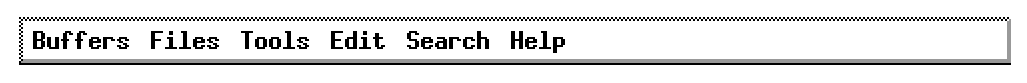
\epsfig{file=ps-files/screen-shot-2.ps, width=\textwidth}
\end{center}
\caption{{\tt emacs} will change its menu bar depending on the type of
  file you're working on.  Here is one possible menu
  bar.}\label{x11-menu-bar}
\end{figure}

\subsection{Scroll Bars}\label{x-scroll-bar}

A {\bf scroll bar} is a method to allow people to display only part of
a document, while the rest is off the screen.  For instance, the {\tt
  xterm} window is currently displaying the bottom third of the text
available in Figure~\ref{x11-scrollbar}.  It's easy to see what part
of the available text is current being displayed: the darkened part of
the scroll bar is relative to both the position and the amount of
displayed text.  If the text displayed is all there is, the entire
scroll bar is dark.  If the middle half of the text is displayed, the
middle half of the scroll bar is darkened.\index{X Window System!scrollbar}

A vertical scroll bar may be to the left or right of the text and a
horizontal one may be above or below, depending the application.

\begin{figure}[tb]
\begin{center}
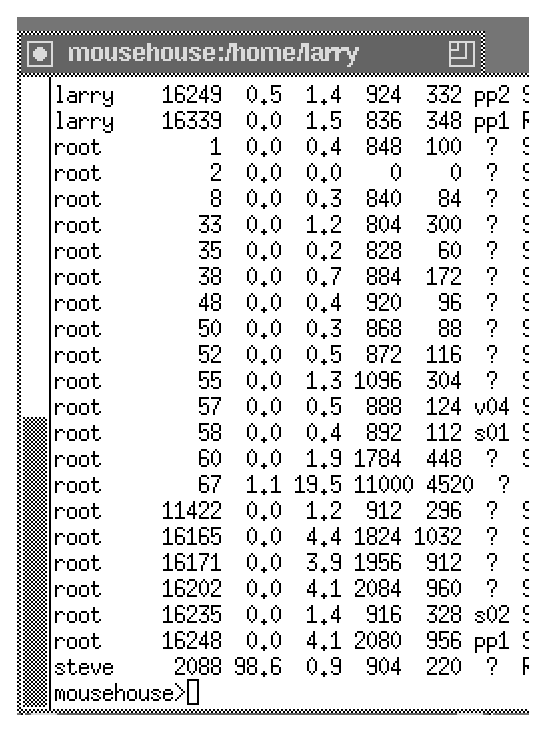
\epsfig{file=ps-files/screen-shot-3.ps, height=3in} \hspace{0.7in}
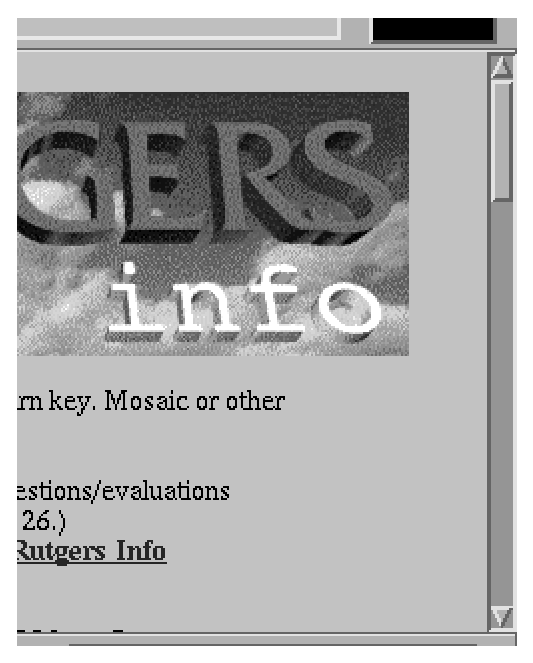
\epsfig{file=ps-files/screen-shot-4.ps, height=3in}
\end{center}
\caption{An Athena-type scroll bar is visible on the left of this {\tt
    xterm} window.  Next to it, a Motif-type scroll bar is visible on
  the {\tt netscape} window.}\label{x11-scrollbar}
\end{figure}


\subsubsection{Athena scroll bars}

Athena scroll bars operate differently from scroll bars in other
windowing systems.  Each of the three buttons of the mouse operate
differently.  To scroll upwards (that is, display material above what
is currently visible) you can click the rightmost mouse button
anywhere in the scroll bar.  To scroll downwards, click the left mouse
button anywhere in the scroll bar.

You can also jump to a particular location in the displayed material
by clicking the middle mouse button anywhere in the scroll bar.  This
causes the window to display material starting at that point in the
document.

\subsubsection{Motif scroll bars}

A Motif scroll bar acts much more like a Microsoft Windows or
Macintosh scroll bar.  An example of one is on the right in
Figure~\ref{x11-scrollbar}.  Notice that in addition to the bar, it
has arrows above and below it.  These are used for fine-tuning:
clicking either the left or middle buttons on them will scroll a small
amount such as one line; the right button does nothing.

The behavior of clicking inside the scroll bar is widely different for
Motif scroll bars than Athena scroll bars.  The right button has no
effect.  Clicking the left button above the current position scrolls
upward.  Similarly, clicking below the current position scrolls
downward.  Clicking and holding the left button \emph{on} the current
position allows one to move the bar at will.  Releasing the left
button positions the window.

Clicking the middle button anywhere on the bar will immediately jump
to that location, similar to the behavior of the Athena middle
button.  However, instead of starting to display the data at the
position clicked, that position is taken to be the \emph{midpoint} of
the data to be displayed.

\eindex{X Window System}
% Local Variables: 
% mode: latex
% TeX-master: "guide"
% End: 
